\documentclass{article}
\usepackage[utf8]{inputenc}
\usepackage{graphicx}
\usepackage{tikz}
\usepackage{todonotes}
\usepackage{hyperref}
\usetikzlibrary{arrows, arrows.meta}
\usepackage{float}
\usepackage[]{algorithm2e}
\usepackage{pgfplots}
\usepackage{minted}

% Use standard A4 paper and standard margins for A4.
\usepackage[a4paper, margin=2.54cm]{geometry}

\begin{document}
\begin{titlepage}
    \begin{center}
       \vspace*{4cm}

       \textbf{\LARGE Tetris Project for AOS}

       \vspace{1.5cm}
        Design Document for the Tetris project for the course "Advanced Operating System".
            
       \vfill

       \textbf{Authors:}\\
       Accordi Gianmarco\\
       Chierici Franco

       \vspace{0.8cm}
     
       
\includegraphics[width=0.4\textwidth]{img/Logo_Politecnico_Milano.png}
            
       Dipartimento di Elettronica, Informazione e Bioingegneria\\
       Politecnico di Milano\\
       Italy\\
       29/03/2021
            
   \end{center}
\end{titlepage}

\tableofcontents

\newpage

\section{Introduction}
The scope of this document is to explain the design choice we have have made during the development of our project: a version of Tetris working from a terminal console, that is executed on an external microcontroller integrated circuit. 
It will also contains all the reference to better understand the structure of the code.

\section{Design}

\subsection{Interfaces Diagram}
\begin{figure}[H]
    \centering
    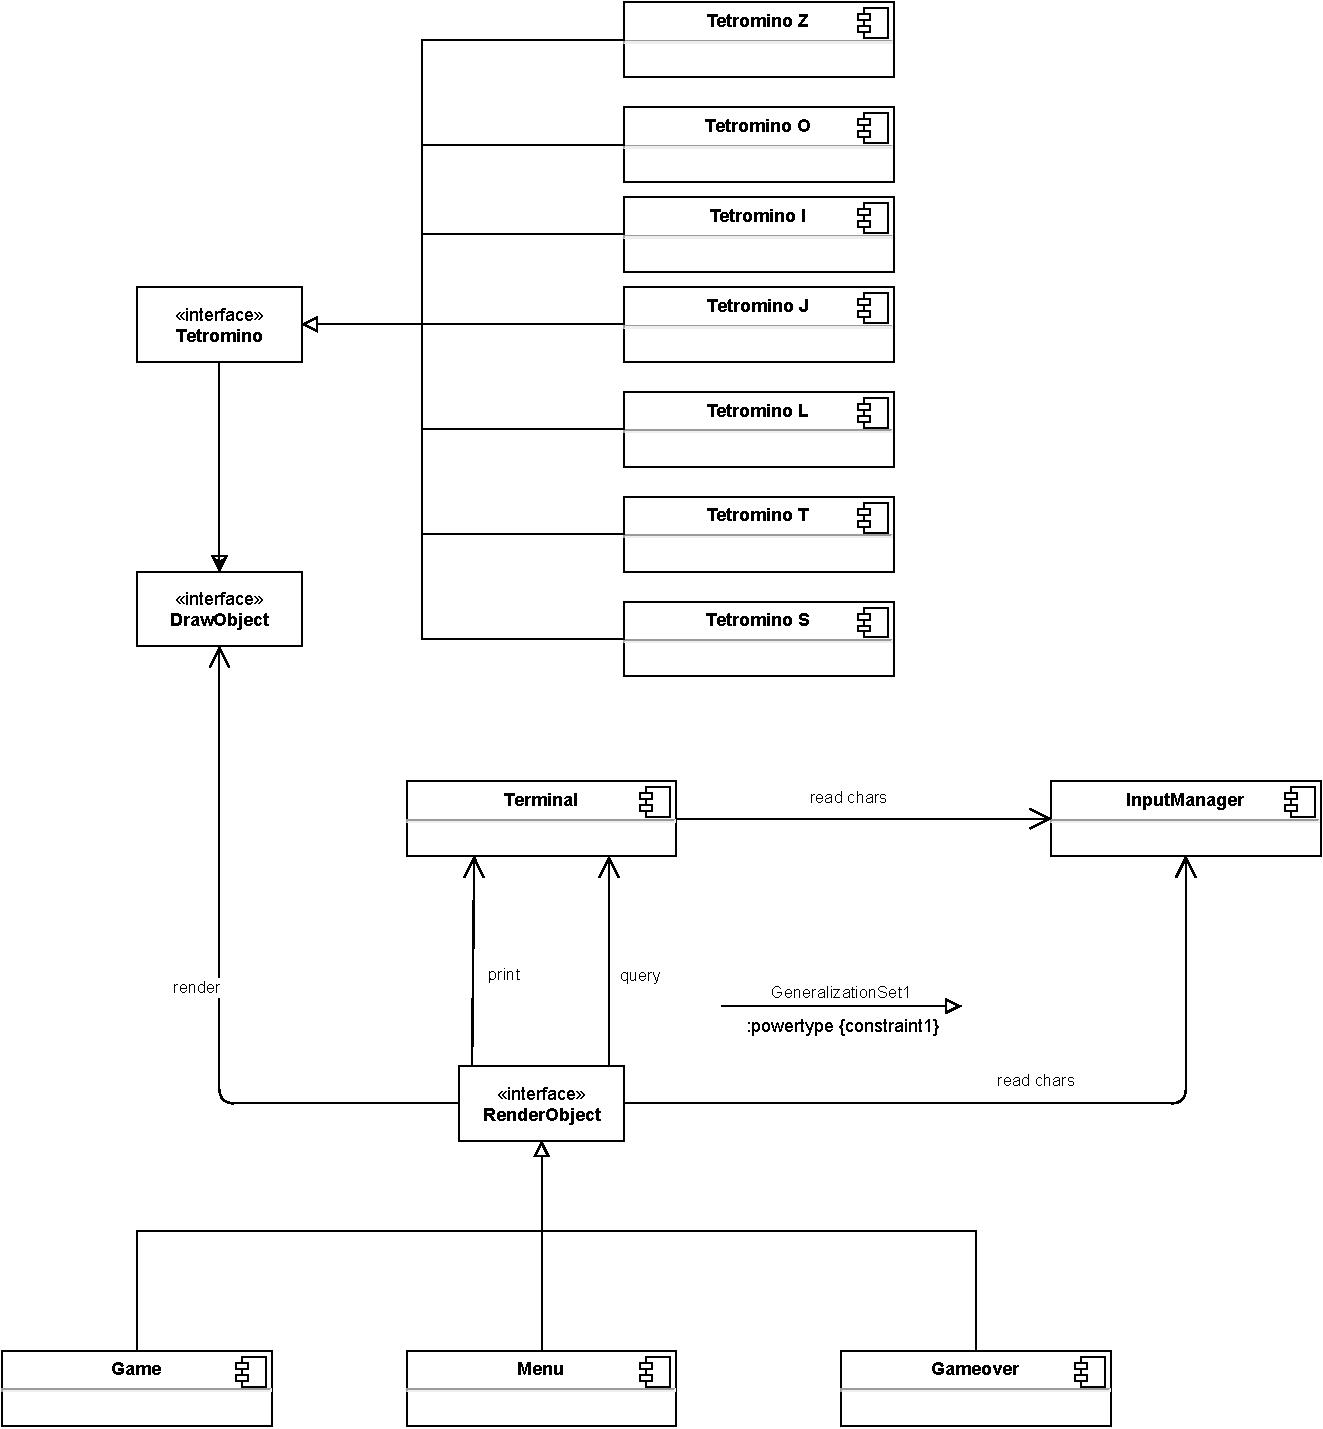
\includegraphics[width=\linewidth]{img/InterafcesDiagram.pdf}
    \caption{Interfaces Diagram of the project.}
    \label{fig:interface}
\end{figure}
The previous diagram \ref{fig:interface} shows the high level structure of project. From it you can see that there are two relevant classes: the \textit{Terminal} and the \textit{InputManager}.
They are two implementation dependent classes that has been introduced in order to decouple the main project logics from the actual platform used.
The \textbf{Terminal} is used to query the terminal used in order to get the available space on the terminal screen, sets the terminal mode, and to print object on it, as further detailed inside \ref{terminal-rendering}.
When needed the following functions are exposed by the Terminal:
\begin{minted}[linenos, bgcolor=white, escapeinside=!!]{c++}
    /* When needed use this method to update the value of col and row */
    int refreshColAndRow();
    /* Set the position of the cursor to the left higher corner of the drawing area, relative
    to the given row and col. */
    void positionCursorForStartDrawing(int posRow, int posCol);
    /* Draw a portion of the screen based on DrawObject
    starting from the position on screen (writingRow, writingCol). */
    void drawOnScreen(DrawObject drawObject, int writingRow, int writingCol);
\end{minted}
The Terminal is instantiate in the entry point of the project that is obviously located at \path{main.cpp}, along with the declaration of the InputManager, than their reference is carried along and passed in the constructor of each
elements that are interested.
The \textbf{InputManager} instead manages the interactions with the user, it collects the characters received from the user in a queue, that is later on read by interested elements (like a \textit{RenderObject}).
\begin{minted}[linenos, bgcolor=white, escapeinside=!!]{c++}
    /* Returns an instance of the last char received from the user.
    NOTE: it is a blocking call. */
    char getLastChar();
    /* Returns an instance of the last char received for the terminal.
    NOTE: it is a blocking call. */
    char getLastCharForTerminal();
\end{minted}
It keeps track of two different queue: one that can be accessed by each element, and the second one only by the terminal. Since we are using ASCII Escape Sequence, we will query the terminal and receive response on the STDIN, so when doing this operation we suspend the adding into the queue of the next char on the STDIN,
and instead we put these chars on the queue for the Terminal, in this way we avoid that the two different streams of chars are mixed altogether.
One of the other Main interfaces is the \textbf{RenderObject}. There will be only one RenderObject at a time, and will be managed by the main code.
As detailed in the \ref{main-loop} each frame we draw is done by calling on the active RenderObject the method:
\begin{minted}[linenos, bgcolor=white, escapeinside=!!]{c++}
    /* Render method of the screen through the Terminal. */
    virtual RenderObject * drawFrame();
\end{minted}
Which draw at each frame what has to be displayed on the screen by the Terminal, that sometimes requires the whole content of the screen to be cleared (call \textit{resetScreen()} on Terminal), or only a portion of it (by using \textit{revertDrawObject()} to undone a previous print, this is done in order to optimize).
The various RenderObject are: \textit{Game}, \textit{Menu}, and \textit{Gameover}.
They all contains the logic used to implement the game.
The other abstraction we have used is to defined the \textbf{DrawObject}, that is an object composed by the following fields:
\begin{minted}[linenos, bgcolor=white, escapeinside=!!]{c++}
    /* Is the string associate to this DrawObject */
    string object_string;
    /* Is the color associate to this DrawObject */
    string color;
\end{minted}
Tha are used by the Terminal when a call to print a DrawObject is done.
The last level of abstraction is represented by the \textbf{Tetromino}, that provides an high level interface, that is extended for each other Tetrominoes. In this way each new Tetrominoes needed requires only to provide a valid constructor that draw the shape of the Tetromino as it was draw on a Grid.
In fact also the state of the Game inside the \textbf{Game} class is saved inside a grid, that when needed is translated inside a DrawObject and sent to the Terminal to be printed.
The definition of the Tetromino class then includes also:
\begin{minted}[linenos, bgcolor=white, escapeinside=!!]{c++}
    /* Returns a string that should be printed on screen. */
    DrawObject toDrawObject();
\end{minted}
that is used in order to get the DrawObject starting from the Tetromino that should be sent to the Terminal to be printed.

\subsection{Sequence Diagram}
\begin{figure}[H]
    \centering
    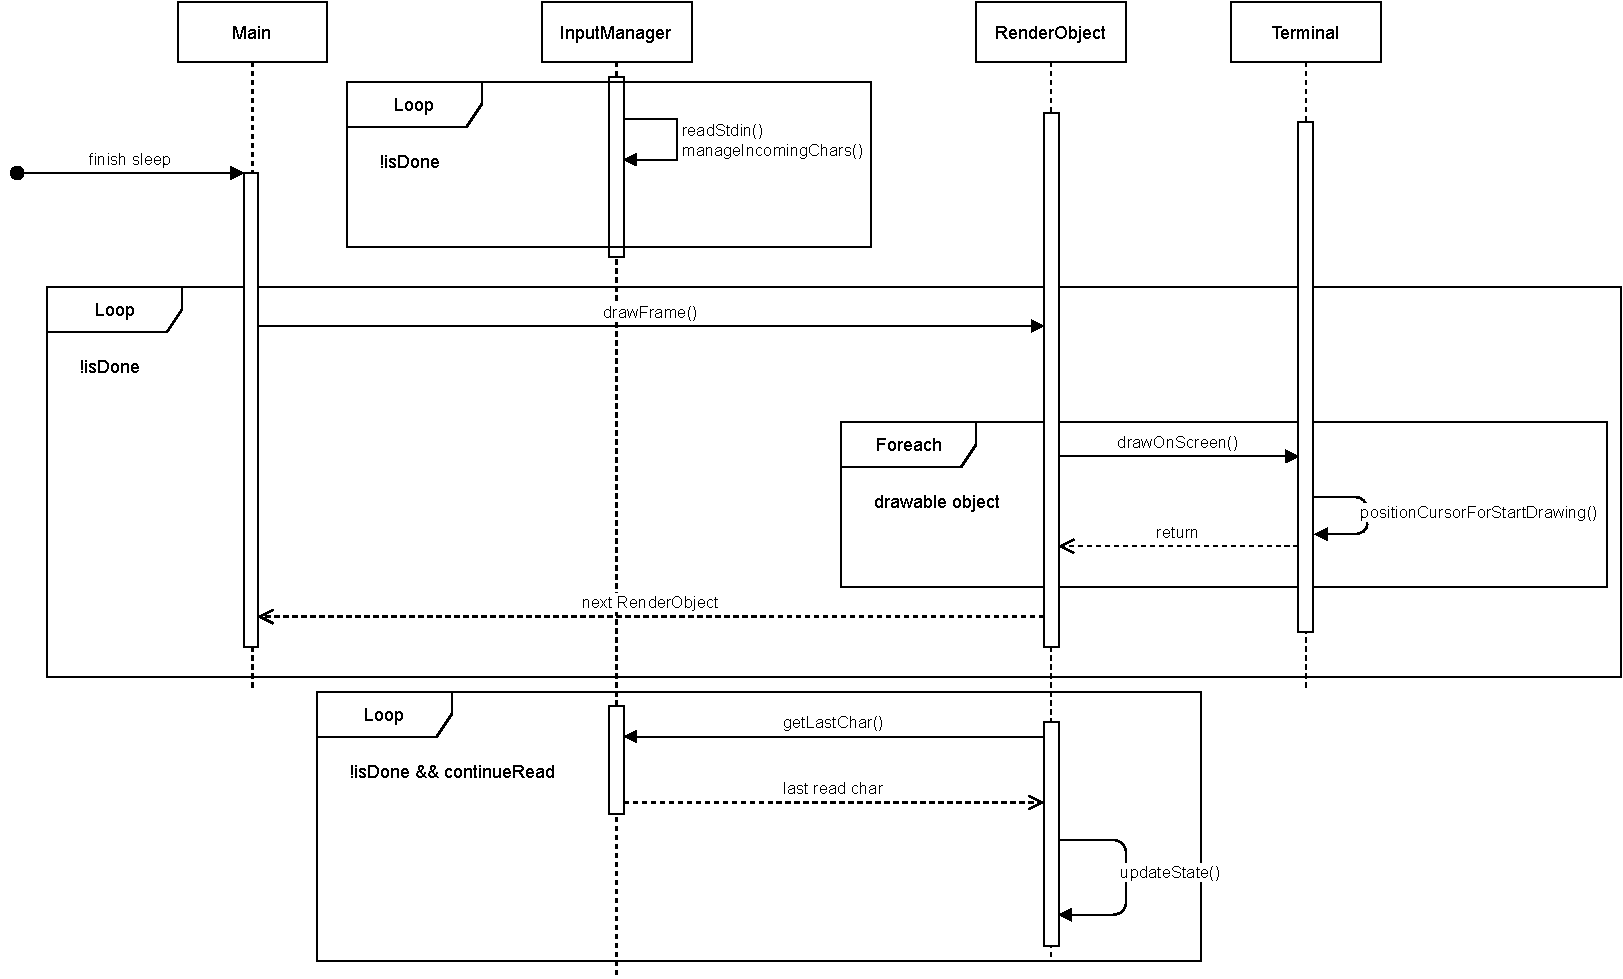
\includegraphics[width=\linewidth]{img/SequenceDiagram.pdf}
    \caption{Sequence Diagram of the project.}
    \label{fig:sequence}
\end{figure}
Talk about isDone

\section{Target Platform}

\section{Implementation}
This part of the document better highlight what hwo we have proceed in the implementation of our project from a more technical perspective.

\subsection{Packages}
Our project has been developed by using C++\cite{slidec++}, in order to be compliant with the miosix-kernel\cite{miosix}.

\subsection{Terminal Rendering}
\label{terminal-rendering}


\subsection{Main Loop}
\label{main-loop}
\begin{algorithm}[H]
    Setup of the InputManager and the Terminal\;
    \While{!isDone} {\
        Synchronized with MPI\_Barrier(MPI\_COMM\_WORLD)\;
        \eIf{myID==processorID}{
            Allocate enough buffer in order to receive from each processor information about the amount of data it will send\;      
        }
        {
            Prepare the information about the amount of data to be sent\;
        }
        Perform an MPI\_Gather\;       
        \eIf{myID==processorID}{
            Allocate enough buffer, based on the information received in the previous gather, in order to receive from each processor the data it will send\;    
        }
        {
            Prepare the data to be sent\;
        }
        Perform an MPI\_Gatherv\;
    }
    \caption{Main loop executed inside the main.cpp.}
\end{algorithm}

\subsection{Development Note}
In order to proceed with the development of our project, we have locally cloned the github repository of the miosix kernel\footnote{https://github.com/fedetft/miosix-kernel}.
After removing the \emph{.git} folder, we have also cloned into the same folder our repository\footnote{https://github.com/gianfi12/AOS-Tetris}.
In order to keep our code more parametric as possible we have defined an header file at \path{terminal/utility.h} that acts as a configuration file 

\section{Usage and Setup}


\bibliographystyle{plain}
\bibliography{references}
\end{document}